\chapter{Results and Analysis}\label{ch:results-and-analysis}
\initial{T}o document the effectiveness of the Pozyx setup results were gathered in several scenarios as seen in Chapter~\ref{ch:design-experiments}.
From a qualitative point, the embedded EKF fusing the dead reckoning data and tag data seems to outperform the other methods in terms of falling close to the actual path and being robust to the erratic behaviour introduced by No Line of Sight.
The plots also highlight a major issue that arose when the tag was in motion and there was No Line of Sight between one of the anchors and the tag.
Although it was easy to pinpoint the major issues from the plots, a quantitative measure was required to solidify the findings.
A useful metric would be to see the distance from the supposed positions to the path being traveled.
Since the robot moved autonomously and there was no perception of where it should be at a given time, a way of effectively measuring the distance to the path needed to be designed.
Figure~\ref{fig:dist} shows what is available while data is being recorded.
The green arrows represent the minimum distance for a candidate point and the path.
Appendix~\ref{app:app04} shows the general pseudo-code to obtain the green distance for each point.
A benefit of using a distance metric is that it is easy to interpret and ideally should be zero if the pose estimates are completely accurate.
This also means that standard statistics on this distance metric would give a clear indication of which method produced the best results.
Table~\ref{tb:results} shows the final metrics obtained for the various results.
The table is color coded to indicate what the inputs to the EKF are for each test.
In addition to the EKF fused results, the statistics for the tag and dead reckoning positions were included to set a benchmark for comparison.
As expected the estimates combining the dead reckoning and tag readings clearly outperforms the others.
The EKF implemented on the WMR is quite simple so it is expected that similar or even better results would be obtained on the FCU whilst in flight.

\begin{figure}[h!]
    \centering
    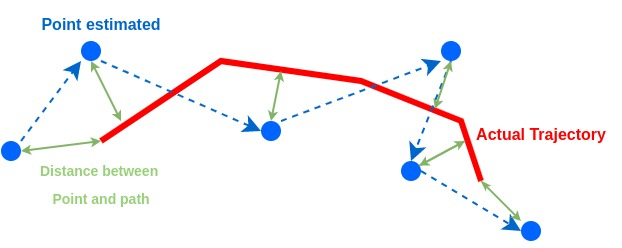
\includegraphics[scale=0.7]{dist_metrics}
    \caption{Illustration of how a distance metric was developed for analysis.}
    \label{fig:dist}
\end{figure}


\begin{table}[h!]
    \centering
    \begin{tabular}{|c|}
        \hline
        LOS = Line of Sight\\
        NLOS = No Line of Sight\\
        EKF = Extended Kalman Filter\\
        WMR = Wheeled Mobile Robot\\
    \end{tabular}
    \begin{tabular}{|c|}
        \hline
        \rowcolor{LightNavy} EKF input is only the Readings of the Pozyx Tag\\
        \rowcolor{LightGreen} EKF input consists of Dead reckoning readings \& Pozyx tag Readings\\
    \end{tabular}
    \begin{tabular}{|c|c|c|c|c|c|}
        \hline
        & Max & Mean & Variance & Skew & Kurtosis \\
        \hline
        \rowcolor{LightNavy}Trajectory 1 traced by human with LOS & 0.4031 & 0.115 & 0.007 & 1.219& 0.5642\\
        \hline
        \rowcolor{LightNavy}Trajectory 2 traced by human with LOS & 0.1563 & 0.06 & 0.0016 &0.1164 & -1.432\\
        \hline
        \rowcolor{LightNavy}Trajectory 2 by WMR with LOS & 0.0795 & 0.04 & 0.0009 & -0.0735 & -1.7372\\
        \hline
        \rowcolor{LightNavy}Trajectory 1 by human with NLOS & 0.331 & 0.114 & 0.006 & 0.7851 & -0.1624\\
        \hline
        \rowcolor{LightNavy}Trajectory 2 by human with NLOS & 0.137 & 0.0431& 0.0009 & 1.0405 & 0.3421\\
        \hline
        \rowcolor{LightNavy}Trajectory 2 by robot with NLOS &  0.3297 & 0.05416 & 0.00189 & 1.0415 & 3.8087\\
        \hline
        \rowcolor{LightGreen}Trajectory 2 by WMR with NLOS & 0.087 & 0.036 & 0.00047 & 0.1634 & -0.2665\\
        \hline
        Raw Dead Reckoning readings & 0.1081 & 0.067 & 0.00136 & -0.9802 & -0.8165\\
        \hline
        Raw Pozyx Tag Readings & 0.1124 & 0.069 & 0.00153 & -0.5188 & -1.352\\
        \hline
    \end{tabular}
    \caption{Metrics for the Distance from each path for different tests and positions.}
    \label{tb:results}
\end{table}
